\section{Introduction}
The Cave eXploration (CaveX) honours project aims to assist researchers in understanding cave systems through an improved ability to create maps of them. This iteration of the project serves to introduce autonomous functionality into the prototype from the project's 2022 iteration, shown in Figure \ref{fig:caveXrobot}. Such an expansion of capability is primarily going to be developed around the use of Light Detection and Ranging (LiDAR) data as it permits autonomous navigation without excessive disturbance of cave environments.

\begin{figure}[H]
    \centering
    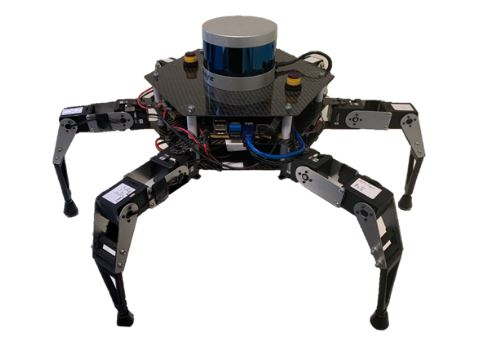
\includegraphics[scale=0.75]{caveX_robot.JPG}
    \caption{The current CaveX hexapod robot prototype, featuring upgraded actuators, a lighter structure, and more robust control software. (Bright et al. 2022)}
    \label{fig:caveXrobot}
\end{figure}

\subsection{Background}
Caves serve as scientific time capsules due to their isolation from the world and minimal human disturbance. Consequently, they are of particular interest to palaeontologists, geologists, and researchers of other scientific fields to better understand important ecological artefacts (Kambesis 2009). Researchers however are often limited by unfavourable cave structures limiting their access to areas (Kambesis 2009). Palaeontologists from The University of Adelaide, Dr Elizabeth Reed and Craig Williams, are currently mapping South Australia’s Naracoorte Caves which involves the mapping of 23 distinct caves, each with unique morphological features (Kambesis 2009). Accurate and detailed maps facilitate an improved understanding of the caves' structures, formation, and composition. Currently, the caves are mapped using a tripod-mounted LiDAR system that is manually moved with human involvement (Bright et al. 2022, p. 1). This system is unfavourable as it is time consuming, too large or cumbersome to scan some parts of the caves, and labour-intensive (Bright et al. 2022, p. 1). Thus, a system which improves on these qualities would considerably improve the quality of research and the rate at which research can be conducted (Bright et al. 2022, p. 1). A system that can also reduce the impact of human presence in natural cave environments is desirable.


The CaveX honours project, started in 2021, intends to create an autonomous biomimetic robot with cave mapping capabilities beyond that of current technologies. In particular, the autonomous system should be able to map difficult-to-reach sections of cave systems to expand researchers’ ability to collect data and complete existing maps of cave systems. To improve the system robustness a gait control system will also be implemented such that the movement of the robot will automatically adjust depending on the type of terrain. Implementing this feature will ensure the robot can adapt to different conditions throughout the cave environment improving its reliability. The current iteration of the robot can traverse cave systems under the control of a human operator but lacks any significant autonomous functionality. Implementing autonomy would not only improve the useability of the prototype but will also improve the system effectiveness and deliver its maximum potential value to researchers.


The robot currently uses a LiDAR sensor to generate a point cloud map of the surrounding cave environment. This point cloud map could also be used as a map to aid the robot in journey planning and autonomous traversal of the local environment. Simultaneous localisation and mapping (SLAM) algorithms are popularly paired with LiDAR data for autonomous movement. The aim of SLAM algorithms is to build maps of the environment surrounding the robot whilst also simultaneously determining the position and orientation of the robot within the map itself (Zou et al. 2022). Utilising the three-dimensional point cloud map produced by a LIDAR sensor allows for depth to be incorporated effectively into the map which makes it advantageous over computer vision navigation two-dimensional images from a camera (Zou et al. 2022).

\subsection{Motivation}
The current method of mapping the Naracoorte caves includes a large tripod mounted LiDAR sensor which is unfavourable in mapping tight cave passages. Previous iterations of the CaveX project have been able to produce a robot which is capable of mapping the cave environment under the control of a human operator. In order to manually control the robot, the operator needs a good understanding of the path the robot will take and needs to be aware of any obstacles in its path. This means that the robot's path is limited to what the operator can see thus effecting the robots effectiveness and robustness. The possibility of finding previously undiscovered cave entrances or formations is also significantly lowered. Autonomous operation of the robot can be implemented into multiple facets of its operation including movement, gait control, path planning and obstacle avoidance.

The current prototype utilises the LiDAR sensor to generate a three-dimensional (3D) point cloud map of the caves interior surface. Autonomous movement can be implemented through machine learning (ML) and artifical intelligence (AI) algorithms integrated into this data from the LiDAR sensor allowing the robot to understand its position in the map. Autonomous movement will allow the robot to move without direct control of the user which extends its utility and breadth of searching in the cave environment. An important milestone to achieving effective autonomous traversal of the cave environment is the ability for the robot to sense the terrain it is on and to adjust its gait accordingly. Different gaits are suited to different surface conditions as they provide the robot with specific measures of speed and stability. Traversing on surfaces with non-optimal gaits can significantly limit the speed of the robot and can also cause it to loose stability. Other complications such as motor stalling can also occur. The robot must also have a path planning capability to plan its next steps for its journey through the cave in real-time. Lastly, the cave system is far from a smooth, obstacle-free environment. This means that the robot must have the ability to detect obstacles and consequently alter its journey to avoid these obstacles. Implemented together, these abilities can supply the robot with an autonomous capability which would greatly improve its operation and value to researchers endeavouring to map the Naracoorte Caves.

\subsection{CaveX Mission Statement}
The 2022 CaveX project team developed a mission statement which is intended to represent the overarching goal for all CaveX project teams.

\textbf{CaveX mission statement:} To design and build a bio-inspired autonomous robot for the purpose of exploration and 3D mapping of cave systems.

The 2023 CaveX project team's aims are consistent with the mission statement. This year's project iteration will specifically focus on implementing an autonomous capability onto the robot. Previous years have not achieved this functionality which is directly mentioned in the CaveX mission statement. 

\subsection{2023 Project Aims, Scope, and Objectives}
\label{aims_scope_objectives}
The aim of the 2023 CaveX project is to introduce autonomous capabilities, improve gait robustness, and real time system monitoring functionality into the prototype developed by the 2022 team to extend its utility in exploration and enable efficient development of the project's future iterations. This is to be achieved via the selection, design, implementation, and testing of software and algorithms on the prototype, as well as minor adjustments to its physical components as needed.

The project scope encompasses using the prototype to autonomously explore caves while collecting LiDAR scans and the production of maps from such data. Analysis and integration of these maps with existing data is intended to be conducted by Craig Williams or another third party. The software improvements are primarily intended to introduce autonomous capabilities into the prototype, although a secondary purpose is to facilitate efficient development and debugging. The intent of any physical modifications is to facilitate the software implementation.

The project's objectives signify specific development milestones and have been developed using the Specific, Measurable, Achievable, Relevant, Time-based (SMART) goal structure. This ensures they are justified, achievable, and meaningful. SMART objectives build a strong foundation for the project timeline, and maintain consistency with the 2022 CaveX project team's development process. The 2023 project objectives are summarised in Table \ref{tab:objectives} and defined comprehensively in Appendix \ref{app:smartobj}.

% table of summarised objectves goes here
\bgroup
\rowcolors{2}{white}{gray!25} % first row in pattern (1st, 3rd, 5th, etc) is gray!25, second row in pattern is white (2nd, 4th, 6th, etc)
\begin{xltabular}{\textwidth}{M{1cm}M{3.2cm}M{5cm}M{3.2cm}M{1.8cm}}
\caption{The project's technical objectives with target completion dates.}\label{tab:objectives}
\\ \hline
\rowcolor{gray!50}
\textbf{ID} & \textbf{Objective Description} & \textbf{Specifications} & \textbf{Deliverables / Outcomes} & \textbf{Target Date}
\\ \hline
\csvreader[late after line = \\, separator = semicolon]{./csv/ob2-1-of-2.csv}{1 = \a, 2 = \b, 3 = \c, 4 = \d, 5 = \e}{\a & \b & {\begin{FlushLeft}\c \end{FlushLeft}} & {\begin{FlushLeft}\d \end{FlushLeft}} & \e}
\end{xltabular}
\egroup

\bgroup
\rowcolors{2}{white}{gray!25} % first row in pattern (1st, 3rd, 5th, etc) is gray!25, second row in pattern is white (2nd, 4th, 6th, etc)
\begin{xltabular}{\textwidth}{M{1cm}M{3.2cm}M{5cm}M{3.2cm}M{1.8cm}}
\hline
\rowcolor{gray!50}
\textbf{ID} & \textbf{Objective Description} & \textbf{Specifications} & \textbf{Deliverables / Outcomes} & \textbf{Target Date}
\\ \hline
\csvreader[late after line = \\, separator = semicolon]{./csv/ob2-2-of-2.csv}{1 = \a, 2 = \b, 3 = \c, 4 = \d, 5 = \e}{\a & \b & {\begin{FlushLeft}\c \end{FlushLeft}} & {\begin{FlushLeft}\d \end{FlushLeft}} & \e}
\hline
\end{xltabular}
\egroup

\subsection{Project Management}
The 2023 CaveX project is managed using using various project management tools. This year's project aims to have an emphasis on quality management and a quality assurance plan is included in Appendix \ref{app:qualityplan}. The quality assurance plan is closely related to the project's risk management which involves identifying project risks and safety risks associated with specific implementation details. Appendix \ref{app:riskmanagement} shows a risk assessment (RA) for project related risks and outlines mitigation strategies which help to ensure a high level of quality is achieved. Risk assessments and safe operating procedures (SOPs) for the safety risks associated with the technical work that has currently been undertaken is also presented in Appendix \ref{app:riskmanagement}. Jira is used to manage breaking down work and allocating tasks to group members which is discussed in Section \ref{agile_software_engineering}.

\subsection{Report Structure}
This report is structured to outline the systems engineering approach undertaken by the team. The problem definition phase in Section \ref{sec:problem-definition} contains an analysis of key project stakeholders, the context of the system, and development of user needs and system requirements. Preliminary research is required to understand the current state of the art for autonomous robot operation using data from a LiDAR scanner, hence a literature review is included in Section \ref{sec:litreview}. The next phase in defining the problem is to analyse the current prototype which includes various preliminary tests to identify issues or areas for improvement, this analysis is shown in Section \ref{subsec:existing-prototype}. A concept design is then presented in Section \ref{sec:prelim-design} which includes implementing algorithms explored in the literature review to achieve the project's technical objectives. To ensure the objectives are met this report also details a completion plan in Section \ref{sec:completion-plan} for implementing all required functionality and a plan for additional hardware upgrades that may become necessary.